\subsection*{A. Alternative result}

Денис, заядлый футбольный болельщик команды <<Walruses United>>, очень переживал, когда не смог посмотреть и даже узнать результаты последних матчей своего любимого клуба в чемпионате. Всё, что он знает, это то, что за победу даётся 3 очка, за ничью --- 1 очко, за поражение --- 0. Выпишите для Дениса все возможные варианты суммарного количества набранных очков за $N$ игр.

\informat{Одно целое число $N$ (от $0$ до $10^4$).}

\outformat{Целые неотрицательные числа, разделенные пробелами, --- варианты суммарного количества очков в порядке строгого возрастания.}

\example{2}{0 1 2 3 4 6}

\excomm{0 очков соответствует двум поражениям, 1 очко --- поражению и ничьей, 2 очка --- двум ничьим, 3 очка --- победе и поражению, 4 очка --- победе и ничьей, 6 очков --- двум победам.}



\subsection*{B. Boolean}

Ali found in Web one interesting quote. So, Richard Burton says, that false friendship, like the ivy, decays and ruins the walls it embraces, but true friendship gives new life and animation to the object it supports. Ali doesn’t know how it can help to solve this problem, but whatever!

\informat{Одно целое положительное число N (от 1 до 25).}

\examplee{14}{true}{1}{false}



\subsection*{C. Car collection}

Надира только что получила стипендию, что, несомненно, является поводом для покупки автомобиля. Поскольку стипендия у Надиры повышенная, то она может позволить себе две машины. Зайдя в автосалон и увидев разнообразие представленных автомобилей, Надира поняла, что непременно хочет машины двух разных марок. А можете ли Вы посчитать, сколько есть у Надиры различных вариантов покупки?

\informat{В первой строке одно целое положительное число $n$ (от $1$ до $10^5$) --- количество марок машин.\\Во второй строке массив целых чисел $a_i$ (от $1$ до $10^4$) --- количество машин $i$-й марки.}

\outformat{Одно целое положительное число --- количество способов выбрать две машины различных марок.}

\example{3 	\newline 3 2 3 }{21}

\excomm{Число способов выбрать одну машину первой марки и одну машину второй марки равно 6, первой и третьей --- 9, второй и третьей --- 6. Следовательно, ответ равен 21.}



\subsection*{D. Domino}

Для расслабления после тяжёлой домашней работы Сатбек любит играть со своим набором домино, исследуя эффект, как ни странно, домино. Костяшки из его набора, в отличие от стандартных, могут иметь разные высоты. Сейчас он расставляет их на одной прямой так, что при взгляде сбоку кажется, что на прямой стоят отрезки, перпендикулярные прямой. Отрезки --- это потому что все доминошки имеют нулевую толщину, что даёт ещё одно отличие от обыкновенных доминошек. Уже приготовившись наблюдать грандиозную цепную реакцию, Сатбек вдруг решил сначала прикинуть, а какое максимальное количество костяшек он может повалить, толкнув только одну из них? Сатбек, конечно, помнит, что падение доминошки высотой $h$ на позиции $a$ направо вызывает падение в эту же сторону всех доминошек, позиции $b$ которых удовлетворяют неравенству $a < b < a + h$. Аналогично, её падение налево вызывает падение налево всех доминошек, позиции $b$ которых удовлетворяют неравенству $a - h < b < a$.

\informat{В первой строке одно целые положительное число $n$ (от $1$ до $10^5$).\\
Далее $n$ строк содержат по 2 числа, разделенных пробелом: $x_i$ (от 0 до $10^6$) --- позиция $i$-й доминошки и $h_i$ (от 1 до $10^5$) --- ее высота.}

\outformat{Одно целое число --- максимальное количество доминошек, которое можно уронить одним касанием.}

\example{%
5	 \newline
0 3	 \newline
1 1  \newline
5 1  \newline
7 7	 \newline
9 1}{3}

\excomm{Чтобы уронить три доминошки, достаточно толкнуть четвертую доминошку влево. Тогда вместе с ней упадут третья и вторая.}



\subsection*{E. Enlarged triangle}

Чтобы отпраздновать попадание в число ста тридцати шести лучших команд Москвы на четвертьфинале ACM ICPC, Илья, по традиции, купил маленький плоский треугольный тортик. Но повод действительно исключительный, а победы великого Лорда Бендтнера следует отмечать только <<датским>> тортом (то есть, тортом с площадью, равной $S$). Выяснилось, что торт не дотягивает до <<датских>> стандартов, поэтому Илья решил увеличить площадь торта. Это он может сделать путём удлинения всех сторон треугольника на одну и ту же величину. На какое число ему нужно увеличить все стороны, чтобы получить <<датский>> торт?

\informat{Четыре целых числа $a$, $b$, $c$ (от 1 до $10^4$) и $S$ (от 1 до $10^9$). Гарантируется, что треугольник со сторонами $a$, $b$, $c$ существует и его площадь менее $S$.}

\outformat{Одно вещественное число --- длина, на которую необходимо увеличить все стороны (с абсолютной погрешностью не более 0.001).}

\example{2 3 4 6}{1.0000}

\excomm{Площадь треугольника со сторонами 2+1=3, 3+1=4, 4+1=5 равна 6.}



\subsection*{F. Footprints}

Сегодня в прямоугольном лабиринте, разделённым на единичные клетки, заблудился Ерулан (Надира из своего уже выбралась). Пока Ерулан искал выход, на один листок он набросал схему лабиринта (вид сверху), а на другой стал записывать свои ходы (R – направо, L – налево, U – вверх, D – вниз). Когда он выбрался, то на радостях потерял первый листок. А сможете ли Вы восстановить минимально возможные размеры лабиринта, в котором заблудился Ерулан, если он даст Вам только второй листок? Кстати, как сказал Ерулан, вход и выход из лабиринта необязательно должны быть на краю лабиринта.

\informat{Строка из символов 'R', 'L', 'D', 'U' длиной от 1 до $10^5$. Ввод заканчивается точкой.}

\outformat{Два целых положительных числа, разделенных пробелом, --- ширина и высота лабиринта.}

\example{RRRDDLL.}{4 3}

\excomm{Лабиринт из примера:}
\begin{center}
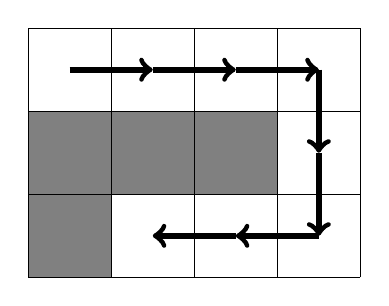
\begin{tikzpicture}[x=30,y=30]
\fill[color=gray](0,0) rectangle (1,2);
\fill[color=gray](1,1) rectangle (3,2);
\draw[step=1] (-0.0,-0.0) grid (4.0, 3.0);

\path[->, draw, line width=2pt] (0.5, 2.5) -- (1.5, 2.5);
\path[->, draw, line width=2pt] (1.5, 2.5) -- (2.5, 2.5);
\path[->, draw, line width=2pt] (2.5, 2.5) -- (3.5, 2.5);
\path[->, draw, line width=2pt] (3.5, 2.5) -- (3.5, 1.5);
\path[->, draw, line width=2pt] (3.5, 1.5) -- (3.5, 0.5);
\path[->, draw, line width=2pt] (3.5, 0.5) -- (2.5, 0.5);
\path[->, draw, line width=2pt] (2.5, 0.5) -- (1.5, 0.5);
\end{tikzpicture}
\end{center}



\subsection*{G. Great divisors}

Темирхан недавно услышал слова британского актёра Ричарда Бёртона о том, что ненастоящая дружба подобно плющу разрушает стены, на которых держится. После этого он не на шутку задумался о том, что каждому созданию нужен настоящий друг. И даже каждому числу! И Темирхан декларировал, что настоящим другом натурального числа будет его максимальный собственный делитель (наибольший делитель, отличный от самого числа). После этого Темирхан решил собрать вместе всех настоящих друзей чисел от 2 до $n$. А какой же отличный способ устроить друзьям веселье, если их просуммировать! Вот Темирхан и нашёл эту сумму. Что же у него получилось?

\informat{Одно целое положительное число n (от 1 до 3 000 000).}

\outformat{Одно целое положительное число --- искомая сумма.}

\example{6}{8}

\excomm{$d_2 + d_3 + d_4 + d_5 + d_6 = 1 + 1 + 2 + 1 + 3 = 8$.}



\subsection*{H. Honest gifts}

Тимур не большой сторонник сладкого, и дарить он предпочитает карандаши. У него есть $a$ красных и $b$ синих карандашей, $k$ из которых он собирается оставить себе, а остальные подарить в виде подарочных наборов. Все подарочные наборы должны быть одинаковыми, то есть, состоять из одного и того же числа красных и синих карандашей. А какое максимальное число наборов он сможет составить?

\informat{Три целых положительных числа разделенных пробелом: $a$, $b$ (от 1 до $10^6$) --- количество красных и синих карандашей соответственно и $k$ (от 1 до $\min(A, B)$) --- количество карандашей, которые Тимур оставляет себе.}

\outformat{Одно целое неотрицательное число --- максимально возможное число наборов.}

\example{27 34 5}{8}

\excomm{Если оставить себе три красных и два синих карандаша, то оставшиеся карандаши можно разбить на 8 наборов по три красных и четыре синих карандаша.}



\subsection*{I. Inner subset}

Александра не большой сторонник канцелярии, и дарить она предпочитает конфеты. У Александры есть $n$ разных коробок, и она знает, что в $i$-ой коробке находится $a_i$ конфет. Она хочет сделать подарок $k$ одногруппникам, поэтому суммарное количество подаренных конфет должно делиться на $k$, но при этом ей нельзя открывать коробки --- это за неё сделают голодные до сладкого студенты. Спрашивается, сколько способов накормить своих друзей есть у Александры? Кстати, она не прочь отдать ребятам даже пустые коробки, если такие будут.

\informat{В первой строке одно целое положительно число $n$ (от 1 до 1000) --- количество коробок.\\ Во второй строке $n$ целых чисел $a_1$, …, $a_n$ (от 0 до $10^9$) разделенных пробелами, где $a_i$ --- количество конфет в $i$-й коробке.\\ В третьей строке целое положительное число $k$ (от 1 до 1000) --- количество одногруппников.}

\outformat{Одно целое неотрицательное число --- ответ на задачу по модулю $10^9 + 7$.}

\example{%
4 		\newline 
1 2 3 4 \newline
3		}{6}

\excomm{В данном случае подойдут следующие варианты: \{~\}, \{1,~2\}, \{3\}, \{1,~2,~3\}, \{2,~4\}, \{2,~3,~4\}.}
